\chapter{ICS Cyberdefense}

A single security product, technology or solution cannot adequately protect an ICS
by itself
A multiple layer strategy involving two (or more) different overlapping security
mechanisms  ---defense-in-depth--- is desired so that the
impact of a failure in any of the mechanisms involved is minimized.

Lo más importante es separar la red corporativa de la red industrial.
\note{Providing logical separation between the corporate and ICS networks
(e.g., stateful inspection firewall(s) between the networks, unidirectional
gateways)}.
Employing a DMZ network architecture (i.e., prevent direct traffic between
the corporate and ICS networks), exploiting, for example, a firewall between the two networks.

% ---

\section{ICS Security Architecture}

\begin{paracol}{2}
   ICS possible attack vectors:
   \begin{itemize}
      \item Backdoors and holes in network perimeter
      \item Vulnerabilities in common protocols
      \item Attacks on field devices
      \item Database attacks
      \item Communications hijacking and `man-in-the-middle' attacks
      \item Spoofing attacks
      \item Attacks on privileged and/or shared accounts
   \end{itemize}
   
   \switchcolumn
   Major security objectives for an ICS security architecture implementation should include the following:
   \begin{itemize}
	\item Restricting logical access to the ICS network and network activity
	\item Restricting physical access to the ICS network and devices
	\item Protecting individual ICS components from exploitation
	\item Restricting unauthorized modification of data
	\item Detecting security events and incidents
	\item Maintaining functionality during adverse conditions
	\item Restoring the system after an incident
   \end{itemize}
\end{paracol}


\subsection{Defense-in-depth}
A single security product, technology or solution cannot adequately protect an ICS
by itself. 
A multiple layer strategy involving two (or more) different overlapping security
mechanisms, a technique also known as defense-in-depth, is desired so that the
impact of a failure in any one mechanism is minimized:
\begin{itemize}
	\item Firewalls
	\item DMZs
	\item IDS
	\item Incident response mechanisms
	\item Physical security and access control
	\item Staff education and training
\end{itemize}

Para garantizar una protección adecuada de los sistemas ICS, es fundamental desarrollar políticas de seguridad, procedimientos y materiales formativos y educativos específicamente diseñados para estos entornos. Estas políticas deben formularse considerando los diferentes niveles de amenaza a los que puede estar expuesto el ICS. Un enfoque eficaz requiere que la seguridad se aborde durante todo el ciclo de vida del sistema: desde la fase inicial de diseño de la arquitectura, pasando por el aprovisionamiento, la instalación y el mantenimiento, hasta el desmantelamiento final. Un elemento crucial de esta estrategia consiste en implementar una topología de red estratificada, donde las comunicaciones más críticas ocurren en el nivel más seguro y fiable, reduciendo así el riesgo de comprometer los procesos esenciales.
\begin{itemize}
	\item Providing logical separation between the corporate and ICS networks
	
   \note{e.g., stateful inspection firewall(s) between the networks, unidirectional
gateways}
	\item Employing a DMZ network architecture
   \note{(i.e., prevent direct traffic between the corporate and ICS networks)}
	\item Ensuring that critical components are redundant and are on redundant networks
	\item Designing critical systems for graceful degradation (fault tolerant) to prevent catastrophic cascading events
	\item Disabling unused ports and services on ICS devices after testing to assure this will not impact ICS operation
	\item Restricting physical access to the ICS network and devices
	\item Restricting ICS user privileges to only those that are required to perform each person’s job (i.e., establishing role-based access control and configuring each role based on the principle of least privilege)
	\item Using separate authentication mechanisms and credentials for users of the ICS network and the corporate network (i.e., ICS network accounts do not use corporate network user accounts)
	\item Using modern technology, such as smart cards for Personal Identity Verification (PIV)
	\note{Regularizar acceso físico es fundamental}
	\item Implementing security controls such as intrusion detection software, antivirus software and file integrity checking software
	\item Applying security techniques such as encryption and/or cryptographic hashes to ICS data storage and communications where determined appropriate
	\item Expeditiously deploying security patches after testing all patches under field conditions on a test system if possible, before installation on the ICS
	\item Tracking and monitoring audit trails on critical areas of the ICS
	\item Employing reliable and secure network protocols and services where feasible
\end{itemize}

\subsection{Network Segmentation and segregation}

\begin{enumerate}
   \item Corporate and ICS must be separated, at least, by a firewall and a
DMZ
   \item Connections between corporate and ICS network must be
minimized
   \item Servers containing the data from the ICS that needs to be
accessed from the corporate network must be put on DMZ
segment
   \item Minimum access should be permitted through the firewall, including
opening only the ports required for specific communication
\end{enumerate}

\begin{paracol}{2}
   \colfill
   
   DMZ  (demilitarized zone) is a network segment that is isolated from the corporate
   network and the ICS network, but is accessible from both. The DMZ is used to
   provide a buffer between the corporate network and the ICS network. The DMZ
   is typically used to host servers that need to be accessed from both the corporate
   network and the ICS network, such as web servers, email servers, and DNS
   servers. The DMZ is also used to host servers that need to be accessed from
   the Internet, such as web servers and email servers. 
   Some considerations:
   \begin{itemize}
      \item The DMZ should be connected to the firewall such that specific
      \item restricted) communication may occur between only the corporate
   network and the DMZ, and the ICS network and the DMZ
      \item The corporate network and the ICS network should not
   communicate directly with each other
      \item Creating a DMZ requires that the firewall offer three or more
   interfaces, rather than the typical public and private interfaces
   \end{itemize}

   \colfill
   \switchcolumn

   \begin{figure}[htbp]
      \centering
      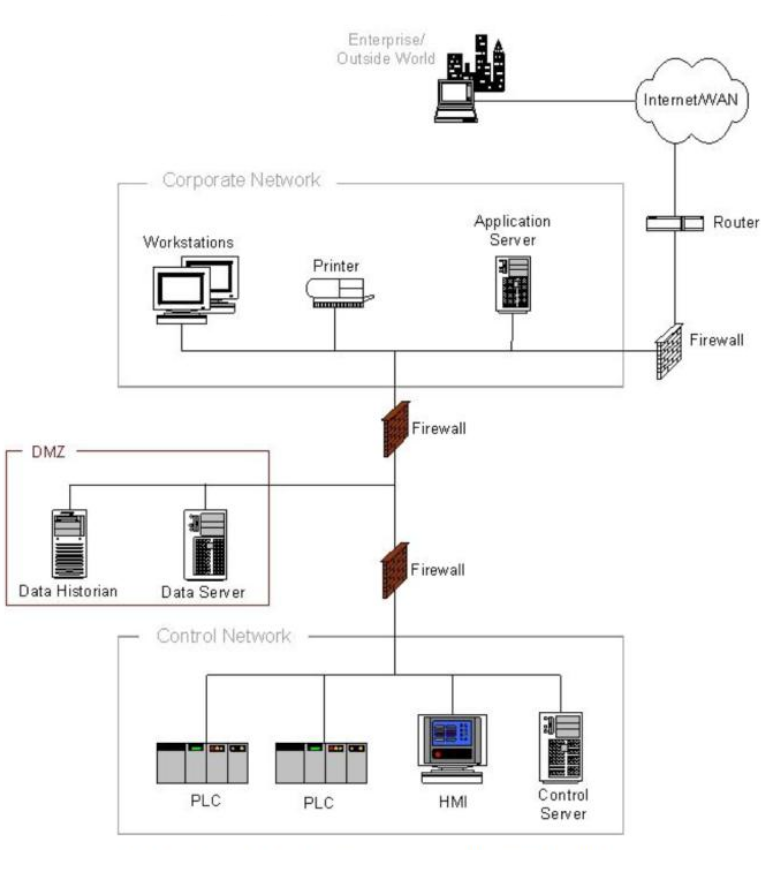
\includegraphics[width=0.90\columnwidth]{images/08/segmentation.png}
      \caption{Segmentation and segregation example}
      \label{fig:08/segmentation}
   \end{figure}
\end{paracol}

Segmentation alternatives:
\begin{itemize}
	\item Physical network separation to completely prevent any interconnectivity of traffic between domains
	\item Logical network separation enforced by encryption or network device-enforced partitioning
\begin{itemize}
	\item VLANs
	\item VPNs
	\item Unidirectional gateways (diodes)
\end{itemize}
	\item Network traffic filtering
\begin{itemize}
	\item IP and route information
	\item Port and/or protocol level filtering
	\item State-based filtering
	\item Application filtering
\end{itemize}
\end{itemize}

Final recommendations to implement a defense-in depth by mean of segmentation
and segregation:
\begin{enumerate}
	\item Apply it at more than just the network layer
	\item If a system doesn’t need to communicate with another system, it should not be allowed to. 
	In such case, there should no possible \textit{physical} path for the communication to occur.
	\item If a system needs to talk only to another system on a specific port or protocol and nothing else, it should be restricted as such.
	\note{Whitelisting over blacklisting}
	\item The most critical components require more strict isolation from other components
	\item Implement whitelisting instead of blacklisting
	\item Denying communications traffic by default and allowing communications traffic by exception
	\item Extending the DMZ concept to other separate subnetworks
\end{enumerate}

\subsection{Firewalling}

There are three types of firewalls: \textit{Packet filtering}, \textit{stateful inspection}, and \textit{application-proxy} firewalls.

Primarily, firewalls are used to protect Internet connections; however, firewalls have applicability also in ICS network environments that do \textit{not} include or require Internet connectivity:
\begin{itemize}
   \item \ul{To restrict connectivity to and from internal ICS networks servicing more sensitive} or criticality functions
	\item \ul{To restrict ICS inter-subnetwork communications} between functional security subnets and devices
\end{itemize}


In an ICS environment, firewalls are most often deployed between the ICS network and the corporate network, to:
\begin{enumerate}
	\item Block all communications with the exception of specifically enabled communications between devices on the unprotected LAN and protected ICS network
	\item Enforce secure authentication of all users seeking to gain access to the ICS network
	\item Enforce destination authorization: Users can be restricted and allowed to reach only the nodes on the control network necessary for their job function
	\item Record information flow for traffic monitoring, analysis, and intrusion detection
\end{enumerate}

Special considerations about firewalls use in ICS environments:
\begin{enumerate}
	\item The possible addition of \textbf{delay} to control system communications
	\item Using firewalls on an individual device basis can create significant management \textbf{overhead}, not permissible in control networks
	\item Firewalls should be \ul{configured so they do not permit either incoming or outgoing traffic by \textit{default}}
	\item By safety, real-time monitoring of firewalls and other security sensors is required to rapidly detect and initiate response to cyber incident
\end{enumerate}

\section{ICT Risk Assessment and Analysis}
The impact of a cyber incident in an ICS may include both digital and physical effects. \textbf{Risk assessments} in ICS need to incorporate those potential effects, while \textbf{safety} is the major consideration that directly affects decisions on how
ICS are engineered and operated.

\begin{definition}
   [Safety]
Safety can be defined as ``freedom from conditions that can cause death, injury, occupational illness, damage to or loss of equipment or property, or damage to the environment.''
\end{definition}


Another major concern for ICS operators is the availability of services
provided by the ICS.
The ICS may be part of critical infrastructure (for example, water or power
systems), where there is a significant need for continuous and reliable operations.
These two concerns must be kept in mind to implement a risk assessment framework in ICS.
\coolquote{ICS may have strict requirements for
availability or for recovery}{Manuel}

Most of ICS engineers and decisión makers will consider that safety and availability are more relevant for ICS than cybersecurity\dots it could be a big mistake\dots and also quite dangerous.

It is important to incorporate the effect of a ICS incident impact on the physical process/system, on dependent systems/processes and, on the physical environment among other possibilities, especially when ICS is part of a critical infrastructure.

The nature of ICS means that there are additional considerations that do not exist
when doing a risk assessment of a traditional IT system:
\begin{itemize}
	\item Impacts on safety
	\item Physical impact of a cyber incident on an ICS, including the larger physical environment; effect on the process controlled, and the physical effect on the ICS itself
	\item Physical disruption of an ICS process
	\item The consequences for risk assessments of non-digital control components within an ICS.
\end{itemize}


Impact of physical disruption of an ICS process:
\begin{itemize}
	\item An incident that impacts the ICS and disrupts the dependent process may
cause cascading impacts into other related ICS processes
	\item Impact to related ICS processes could include both systems and processes
within the organization or systems and processes external to the
organization
	\item Damage to the ICS or physical plant may cause either short or long term
outages depending on the degree of the incident
\note{ An example of a cyber incident impacting the ICS is the Stuxnet malware, which caused physical damage to the centrifuges as well as disrupting dependent processes}
\end{itemize}

Final considerations:
\begin{itemize}
	\item Safety systems may also reduce the impact of a cyber incident to the ICS
	\item Safety systems are often deployed to perform specific monitoring and
control functions to ensure the safety of people, the environment, process,
and ICS
	\item These safety system could mitigate a ICS cybersecurity incident impact
	\item Evaluating the impact of an incident must also incorporate how the impact
from the ICS could propagate to a connected ICS or physical system
	\item Impact propagation could occur due to both physical and logical
dependencies
	\item This situation is known as “Cascade Effect”, and it is very dangerous in the
case of ICS incidents in critical infrastructure
\end{itemize}


\section{Security Control Implementation}

\labelitemize{
   \textit{Access Control}
}{
   \begin{itemize} 	
      \item Access control technologies are filter and blocking technologies designed to direct and regulate the flow of information between devices or systems once authorization has been determined 	
      \item Role-based Access Control (RBAC) should be used to restrict ICS user privileges to only those that are required to perform each person's job (i.e., configuring each role based on the principle of least privilege) 	
      \item Legacy ICS systems or specialized ICS equipment may require development of specialized interface software for access control due to they use a number of proprietary operating systems or customized operating system implementations and interface
   \end{itemize}
}

\begin{itemize}
	\item VLANs are effectively deployed in ICS networks, with each
automation cell assigned to a single VLAN to limit unnecessary
traffic flooding and allow network devices on the same VLAN to
span multiple switches
	\item The general recommendation is to use a one-to-one relationship
between subnets and VLANs
	\item Switches have been susceptible to attacks such as MAC spoofing,
table overflows, and attacks against the spanning tree protocols,
depending on the device and its configuration
\end{itemize}

// TODO

\subsection{Identificación y Autenticación}
\begin{itemize}
	\item Computer systems in ICS environments typically rely on
traditional passwords for authentication
	\item Control system suppliers often supply systems with default
passwords
	\item These passwords are factory set and are often easy to guess or
are changed infrequently, which creates additional security risks
	\item Protocols currently used in ICS environments generally have
inadequate or no network service authentication
	\item Challenge/response authentication may not be feasible for
control system due to the possible latency that may be
introduced
   \item There are now several forms of authentication available in addition to
traditional password techniques being used with ICS
\begin{itemize}
	\item Traditional physical lock and keys
	\item Security cards (e.g., magnetic, smart chip, optical coding)
	\item Radio frequency devices in the form of cards, key fobs, or mounted
tags
	\item Dongles with secure encryption keys that attach to the USB, serial,
or parallel ports of computers
	\item One-time authentication code generators (e.g., key fobs).
	\item Smart Card Authentication
	\item Biometric Authentication
\end{itemize}
\end{itemize}


Disaster Recovery Planning:
\begin{enumerate}
	\item Required response to events or conditions of varying duration
and severity that would activate the recovery plan.
	\item Procedures for operating the ICS in manual mode with all
external electronic connections severed until secure conditions
can be restored.
	\item Roles and responsibilities of responders.
	\item Processes and procedures for the backup and secure storage of
information.
	\item Complete and up-to-date logical network diagram.
	\item The security plan should define a comprehensive backup and
restore policy
\end{enumerate}

Audit and Accountability:
\begin{enumerate}
	\item It is necessary to determine that the system is performing as intended
	\item Traditionally, the primary basis for audit in IT systems has been
recordkeeping
	\item Many of the process control devices that are integrated into the ICS have
been installed for many years and do not have the capability to provide
the audit records
	\item The critical tasks in managing a network in an ICS environment are
ensuring reliability and availability to support safe and efficient operation
	\item Monitoring of sensors, logs, Intrusion Detection Systems (IDS), antivirus,
patch management, policy management software, and other security
mechanisms should be done on a real-time basis where feasible
\end{enumerate}

Intrusion Detection and Prevention:
\begin{itemize}
	\item By mean of IDS, as HIDS an NIDS
	\item In a ICS, NIDS are useful to detect attacks at corporate network and
DMZ segment
	\item Less useful inside control network due to less knowledge about SCADA
attacks network patterns
	\item HIDS are more useful in regular OS computers and servers at corporate
an DMZ networks, due to control devices use (usually) legacy OS, with
bit limitationn in CPU and memory
\end{itemize}
The best way to detect intrusions inside control network is a good
characterization of ``normal'' traffic to detect suspicious changes in it,
denoting attacks. This is especially true for ICS environments, because the traffic is generated by automated applications with little human interaction, making it very predictable.

\begin{itemize}
	\item A patch may remove a vulnerability, but it can also introduce a greater
risk from a production or safety perspective
	\item Patching the vulnerability may also change the way the OS or application
works with control applications, causing the control application to lose
some of its functionality
	\item Another issue is that many ICS utilize older versions of operating
systems that are no longer supported by the vendor, then available
patches may not be applicable
	\item Patching should be scheduled to occur during planned ICS outages, and
previously tested in a similar system out of production mode
\end{itemize}